\documentclass[12pt]{article}
\usepackage{fullpage,amsfonts,amssymb,epsfig,amsmath,hyperref,mdframed, graphicx}
\usepackage{caption, parskip, array}
\newenvironment{gamequote}
               {\list{}{\rightmargin0pt\relax}\item\relax}%
               {\endlist}

\newcommand{\half}{{1 \over 2}}
\newcommand{\xor}{{\oplus}}
\newcommand{\owf}{f}
\newcommand{\Sign}{\mathsf{Sign}}
\newcommand{\Verify}{\mathsf{Verify}}
\newcommand{\KeyGen}{\mathsf{KeyGen}}
\newcommand{\pk}{\mathit{pk}}
\newcommand{\adv}{\mathcal{A}}
\newcommand{\bdv}{\mathcal{B}}
\newcommand{\deq}{\mathrel{:=}}
\newcommand{\rgets}{\mathrel{\mathpalette\rgetscmd\relax}}
\newcommand{\rgetscmd}{\ooalign{$\leftarrow$\cr
    \hidewidth\raisebox{1.2\height}{\scalebox{0.5}{\ \rm R}}\hidewidth\cr}}
\newcommand{\Z}{\mathbb{Z}}
\newcommand{\F}{\mathbb{F}}
\newcommand{\R}{\mathbb{R}}
\newcommand{\G}{\ensuremath{\mathbb{G}}}
\newcommand{\GG}{\ensuremath{\mathbb{G}}}
\newcommand{\Zq}{\ensuremath{{\Z_q}}}
\newcommand{\sk}{\textrm{sk}}
\newcommand{\vk}{\text{vk}}
\newcommand{\lcat}{\langle}
\newcommand{\rcat}{\rangle}
\newcommand{\tuple}[1]{\lcat #1 \rcat}
\newcommand{\KK}{\mathcal{K}}  % key space
\newcommand{\XX}{\mathcal{X}}  % key space
\newcommand{\YY}{\mathcal{Y}}  % key space
\newcommand{\CC}{\mathcal{C}}  % key space
\newcommand{\MM}{\mathcal{M}}  % key space

\newcommand{\FlowRight}[2][200pt]{%
  \xrightarrow{\text{\normalsize\hbox to #1{\hfill \(#2\) \hfill}}}
}
\newcommand{\FlowLeft}[2][200pt]{%
  \xleftarrow{\text{\normalsize\hbox to #1{\hfill \(#2\) \hfill}}}
}


%%%%%%%%
\usepackage{enumitem}

\newenvironment{problems}
{\begin{enumerate}[label=\bfseries Problem \arabic*.,align=left,leftmargin=1em,labelwidth=1.5em]}
{\end{enumerate}}

\newenvironment{subparts}
{\begin{enumerate}[label=\bfseries \alph*.,align=right,leftmargin=1.5em]}
{\end{enumerate}}
%%%%%%%%

\begin{document}

\newlength{\boxwidth}
\setlength{\boxwidth}{\textwidth}
\addtolength{\boxwidth}{-2cm}
\framebox[\textwidth]{
\begin{minipage}[t]{\boxwidth}
{\bf CS155: Computer and Network Security \hfill Spring 2023}  \\[-0.3cm]
\begin{center} {\huge Homework \#1} \end{center}
Due: Thursday, Mar. 27, 2023, by Gradescope.
\end{minipage}}

\vspace{0.7cm}
\begin{problems}

%%%%%%%%%%%%%%%%%%%%%%%%%%%%%%%%%%%%%%%%%%%%%%%%%%%%%%%%%%%%%%
\item \textbf{Jump Oriented Programming (JOP)}

Elizabeth is attacking a buggy application. She has found a vulnerability that allows her to control the values of the registers ecx, edx, and eip, and also allows her to control the contents of memory locations 0x9000 to 0x9014. She wants to use return-oriented programming, but discovers that the application was compiled without any ret instructions! Nonetheless, by analyzing the application, she learns that the application has the following code fragments (gadgets) in memory: \\
\begin{verbatim}
0x3000: add edx, 4      ; edx = edx + 4
        jmp [edx]       ; jump to *edx

0x4000: add edx, 4      ; edx = edx + 4
        mov eax, [edx]  ; eax = *edx
        jmp ecx         ; jump to ecx

0x5000: mov ebx, eax    ; ebx = eax
        jmp ecx         ; jump to ecx

0x6000: mov [eax], ebx  ; *eax = ebx
        ...             ; don't worry about what happens after this
\end{verbatim}

Show how Elizabeth can set the values of the registers and memory so that the vulnerable application writes the value 0x2222 to memory address 0x8888.

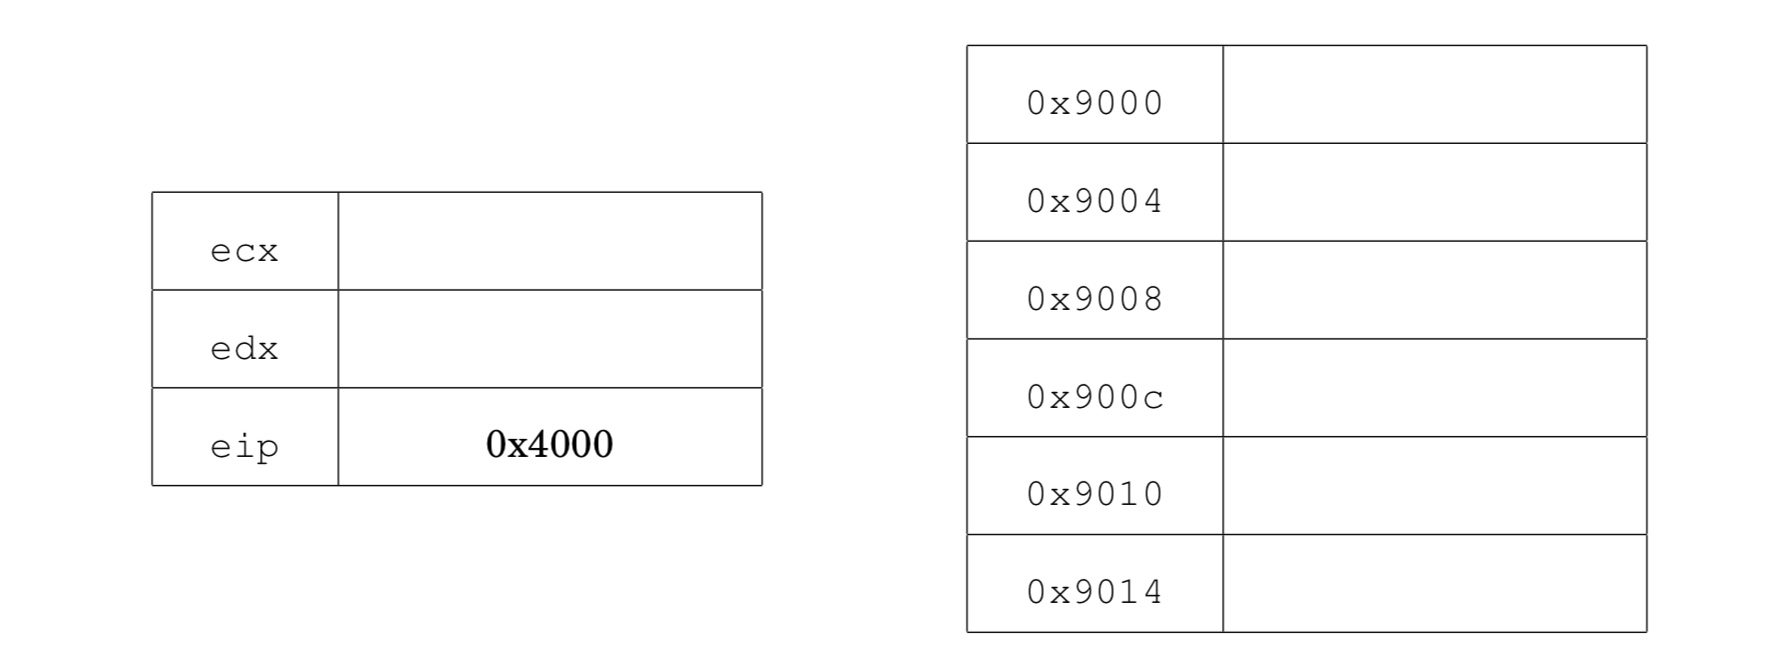
\includegraphics[scale=0.2]{jmp.jpg}

Recall that \texttt{eip} is the instruction pointer. It holds the address of the next instruction to execute. \texttt{ecx} and \texttt{edx} are general purpose registers.

\begin{mdframed}

    Idea: xx

\end{mdframed}

\begin{table}[!htb]
    \begin{minipage}{.5\linewidth}
      \caption{registers}
      \centering
        \begin{tabular}{|l|l|}
            \hline
            ecx & 0x3000 \\ \hline
            edx & 0x9000 \\ \hline
            eip & 0x4000 \\ \hline
        \end{tabular}
    \end{minipage}%
    \begin{minipage}{.5\linewidth}
      \centering
        \caption{stack memory}
        \begin{tabular}{|l|l|}
            \hline
            0x9000 &        \\ \hline
            0x9004 & 0x2222 \\ \hline
            0x9008 & 0x5000 \\ \hline
            0x900c & 0x4000 \\ \hline
            0x9010 & 0x8888 \\ \hline
            0x9014 & 0x6000 \\ \hline
        \end{tabular}
    \end{minipage} 
\end{table}

%%%%%%%%%%%%%%%%%%%%%%%%%%%%%%%%%%%%%%%%%%%%%%%%%%%%%%%%%%%%%%

\newpage

\vspace{1cm}
\item \textbf{Stack canaries}
\begin{subparts}
\item

Recall that when GCC is used to compile a C program with the \texttt{-fstack-protector flag}, the compiler places a stack canary in (almost) every stack frame, and re-orders the local variables. This flag implements a variant of ProPolice discussed in \href{https://cs155.stanford.edu/lectures/02a-ctrl-hijacking.pdf#page=20}{slide 20 in lecture 3}. Write a short sample C program that takes command line input and is vulnerable to a stack smashing attack (i.e., an attack the causes the return address on the stack to be overwritten) even when the program is compiled using GCC with the \texttt{-fstack-protector} flag enabled. \\

Hint: your code could contain a structure that is allocated on the stack, and the structure contains two fields: a pointer and a string. You may assume that the fields of the structure are allocated consecutively on the stack, with the first field allocated at a lower memory address than the second field. An overflow of the string buffer will overwrite the pointer in the structure. Your code should make it possile for the attacker to use that to overwrite entries on the stack.

\item
Suppose the OS marks all stack memory pages as non-executable. Can stack smashing be used to mount a control hijacking attack? If so, briefly explain how. If not, explain why not.

\end{subparts}


\begin{mdframed}
TODO: ANSWER
\end{mdframed}


\newpage
%%%%%%%%%%%%%%%%%%%%%%%%%%%%%%%%%%%%%%%%%%%%%%%%%%%%%%%%%%%%%%
\item \textbf{Integer underflow vulnerability}

Consider the following simplified code that was used earlier this year in a widely deployed router:

\begin{verbatim}
uint32_t nlen, vlen;    /*  values in 0 to 2^32-1  */
char buf[8264];

nlen = 8192;
if ( hdr->nlen <= 8192 )
    nlen = hdr->nlen;

memcpy(buf, hdr->ndata, nlen);
buf[nlen] = ':';

vlen = hdr->vlen;
if (8192 - (nlen+1) <= vlen )    /*  DANGER  */
    vlen = 8192 - (nlen+1);

memcpy(&buf[nlen+1], hdr->vdata, vlen);
buf[nlen + vlen + 1] = 0;
\end{verbatim}

If \texttt{hdr->ndata = "ab"} and \texttt{hdr->vdata = "cd"} then this code is intended to write \texttt{"ab:cd"} into \texttt{buf}. Suppose that the attacker has full control of the contents of \texttt{hdr}. Explain how this code can lead to an overflow of the local buffer \texttt{buf}.

\begin{mdframed}
TODO: answer
\end{mdframed}


\newpage
%%%%%%%%%%%%%%%%%%%%%%%%%%%%%%%%%%%%%%%%%%%%%%%%%%%%%%%%%%%%%%
\item \textbf{Privilige escalation}

After poking around your Unix-based system as the user laura, you stumble to find the following file in \texttt{/sbin}:

\texttt{-rwsrwxr-x   1 root laura   234K Apr 01 21:32 ping}

What's the potential security vulnerability? How might you use this file to escalate your privileges to root? (Assume that ping does not have any vulnerabilities in its implementation.) \\

Modern versions of Linux try to prevent this security escalation. What is the defensive behavior? Hint: try creating a file with these permissions on your VM from Project 1, orchestrating your attack, and seeing what happens. \\

\begin{mdframed}
    Laura's single-user group is the group owner, meaning that in this case she has \texttt{rwx} permissions. This allows her to change the \texttt{ping} program to some shellcode and then execute it, which should give her shell access?

    
\end{mdframed}



\newpage
%%%%%%%%%%%%%%%%%%%%%%%%%%%%%%%%%%%%%%%%%%%%%%%%%%%%%%%%%%%%%%
\item \textbf{Android Isolation}
In Android, each app runs in a separate process using a separate user id. From a security standpoint, what is the advantage of assigning separate UIDs instead of using the same UID for all apps?


\begin{mdframed}
    You can get more granular with the security model, meaning that both file ownership and permissions . This adds layers to the defense in depth: if a single app is compromised, the set of files that the app has access to is smaller.

\end{mdframed}


\newpage
%%%%%%%%%%%%%%%%%%%%%%%%%%%%%%%%%%%%%%%%%%%%%%%%%%%%%%%%%%%%%%
\item \textbf{Reducing executable permissions}
After discovering a vulnerability in the \texttt{passwd} utility, the Linux developers have decided that it is too dangerous to conintue to run the utility as root (through setuid). Unfortuantely, there's no Linux capability that lets a process specifically edit \texttt{/etc/shadow}, the file that Linux uses to store password data.

\begin{subparts}
    \item The kernel developers have asked you to devise a new mechanism where the passwd command no longer runs as root, but users can only change their own password and can't change any other users' passwords. Your solution can't change the Linux kernel itself (e.g., introduce a new capability), but the developers have created a new service account passwd that you can use. You can change the ownership, permissions, or setuid bit on any files, but you should note the new configurations in your solution.

    \begin{mdframed}
        TODO: answer
    \end{mdframed}

    \item What's the worst damage that an attacker can do if a new code exploit vulnerability were to be found in passwd after your proposed fix?

    \begin{mdframed}
        TODO: answer
    \end{mdframed}

    \item Does changing who runs the \texttt{passwd} utility meaningfully increase the security of the system? Why or why not? Hint: Think about the contents of the \texttt{/etc/shadow} file.

    \begin{mdframed}
        TODO: answer
    \end{mdframed}


\end{subparts}



\newpage
%%%%%%%%%%%%%%%%%%%%%%%%%%%%%%%%%%%%%%%%%%%%%%%%%%%%%%%%%%%%%%
\item \textbf{Race conditions}
After discovering a vulnerability in the \texttt{passwd} utility, the Linux developers have decided that it is too dangerous to conintue to run the utility as root (through setuid). Unfortuantely, there's no Linux capability that lets a process specifically edit \texttt{/etc/shadow}, the file that Linux uses to store password data.

\begin{subparts}
    \item Suppose this code is running as a setuid root program. Give an example of how this code can lead to unexpected behavior that could cause a security problem. Hint: see lecture 5 slide 19.

    \begin{mdframed}
        TODO: answer
    \end{mdframed}

    \item Suppose the sleep(10) is removed from the code above. Could the problem you identified in part (a) still occur? Please explain.

    \begin{mdframed}
        TODO: answer
    \end{mdframed}

    \item How would you fix the code to prevent the problem from part (a)? Hint: look up the meaning of the flags \texttt{O\_CREAT} and \texttt{O\_EXCL} given as arguments to the \href{https://linux.die.net/man/3/open}{open} Unix system call. 

    \begin{mdframed}
        TODO: answer
    \end{mdframed}
    
\end{subparts}


\newpage
%%%%%%%%%%%%%%%%%%%%%%%%%%%%%%%%%%%%%%%%%%%%%%%%%%%%%%%%%%%%%%
\item \textbf{Setuid}
You're auditing a new webserver and find the following code snippet:

\begin{verbatim}
if (fork() == 0) {
    int socket = socket(":80");
    if (socket == -1) {
       perror("unable to open socket: ");
       exit(-1);
    }
    seteuid(100);
    serve(socket);
}
\end{verbatim}


\begin{subparts}
    \item How can an attacker escalate privileges if there's a bug in the serve function? You can assume that the service account \texttt{www-data} has the UID 100 and exists, and that the process initially is executed as the root user.

    \begin{mdframed}
        Since the process is initially executed as the root user, an attacker could escalate privaleges by replacing \texttt{seteuid(100)} with \texttt{seteuid(0)} (our root UID). We can do this because unprivaleged users can always change EUID back to RUID or SUID (both of which will be root).
    \end{mdframed}

    \item What change can be made to the code to prevent this privilege escalation vulnerability?

    \begin{mdframed}
        To prevent this privalege escalation vulnerability, our programmer only needs to swap \texttt{seteuid(100)} with \texttt{setuid(100)}. This resets EUID, RUID and SUID together, constraining our attacker to only being able to access UID 100 with appropriate privileges. 
    \end{mdframed}

\end{subparts}

\end{problems}
\end{document}